\section{Results and Discussion}

The scope of experiments in this project involve extensive use of AnACor, the prototype software used at beamline I23 for adding an analytical correction to reflections and reflection intensities \cite{Lu}. Previous work from I23 has documented the successes of tomographic reconstruction and segmentation pipelines to determine analytical absorption factors \cite{Kazantsev2021}, while AnACor has only recently become the routine for this.

A recent publication from I23 and Lu \textit{et al.} \cite{Lu2024} introduces the successful application of analytical absorption corrections based on the 3D-reconstructions from X-ray tomography implemented in AnACor. This paper describes two long-wavelength experiments performed on proteins of chlorite dismutase (Cld) and the membrane protein OmpK36 GD; their results indicating that this approach substantially improves data quality 

Since AnACor is still in development, reoccurring errors occasionally limit our ability to complete data processing and the consistency of results. Validation of the outputted results is therefore still necessary at every stage, and further steps are taken when possible to improve reliability.

When samples containing solely the mother-liquor that crystals were grown in were available, tomography data would be collected on these as well as the crystal samples. This is an example of an optional step taken to improve the reliability of calculating absorption factors. The segmentation of loops containing only liquor allow for more reliable thresholds to be applied as there are fewer materials to account for, and therefore the liquor coefficient is expected to be more precise.

Since low-energy tomographic scans are prone to high contrast artefacts which limit visibility in the segmentation, tomography scans, that would follow diffraction experiments collected at or below 3 \unit{keV}, would often be collected at 3.5 \unit{keV} as well as the low energy. Distinguishing between materials in the 3.5 \unit{keV} projections is somewhat easier, and therefore provides better segmentation for the reflection data collected at lower energies.

%Finally ... preliminary tests

\subsection{Preliminary tests on AnACor}



Because the final reflection data heavily relies on the accuracy of absorption factors, the first experiments conducted for this project were a validation of the accuracy of AnACor's pre-process calculations. Theoretical absorption coefficients are given by the reciprocal of the attenuation length, which can be calculated for a material from its chemical formula, density, and the energy in question. The first experiment on AnACor used crystals of ethylene glycol (\ce{(CH2OH)2}) and santovac, a five ring polyphenyl ether (\ce{C30H22O4}), to compare experimentally calculated absorption coefficients from the software with theoretical coefficients.

The experimental coefficients of santovac, published in \cref{santovac_table} in Appendix A2, are within 1.5 \% of the theoretical value for energies between 3 and 4.5 \unit{keV}. This difference, however, appears to grow with energy, with a nearly 7\% difference at 6 \unit{keV}. A similar trend is seen in \cref{ethylene_table} in Appendix A2, with the sudden jump from 1.2 \% at 5 \unit{keV} to 6.3 \% at 6 \unit{keV} for ethylene glycol.

Assessing from the results of these two proteins, AnACor appears to overestimate coefficients at higher energies and similarly underestimates coefficients at lower energies. A possible explanation for the latter is the effect of high contrast at low energies limiting distinctions between materials; this however does not explain the overestimates at higher energies. It is also possible that the calculations do not sufficiently account for the changing dependence of absorption on wavelength, which is less strong at higher energies and would explain the the discrepancies.

A second validation experiment on AnACor involved samples of chlorite dismutase (Cld) and the membrane protein OmpK36 GD. Data on these two samples has already been analysed in Lu \textit{et al.} \cite{Lu} to compare the same approaches for absorption corrections discussed in this work: a \ac{sh} correction, analytical, and a combination of the two. The aim of this subsequent experiment, was to determine the accuracy of the absorption coefficients of crystal and liquor published in this paper. This was assessed with the assumption that the accuracy would correlate to the best possible data quality, where the intensity to uncertainty ratios ($I / \sigma$) peak and the $R_{merge}$ factors are diminished.

Taking the coefficients published in this paper as a reference and varying both in intervals of \pm 10, sets up a variety of possible combinations of coefficient pairs which can together elucidate the optimal amount of variation in both for improving the merging statistics. The coefficients were varied from -20 \% to + 20 \%; after preliminary results were collected, the liquor coefficients were varied a further interval up to + 30 \%, giving a total of 30 possible coefficient variations. %The crystal reference was

The merging statics for all 30 AnACor experiments are shown in \cref{fig:cld_stats} for Cld and in \cref{fig:ompk_stats} for Ompk. The merging statistics of Cld tell a clearer story than that of Ompk: in \cref{fig:cld_stats} the $I/\sigma$ peaks between +10 and +20\% in the crystal factor, and +10\% for liquor; then looking at the R-factors, these values are minimised at the same variation. This indicates to the combination of coefficients that is presumably the most accurate for these materials, as it provides the best merging statistics.

While the differences in the maximum $I/\sigma$ and minimum R factors to their respective values at $\pm0,\pm0$ are small, in a perfect experiment these optimal statistics would align at $\pm0,\pm0$, as this would indicate that the references AnACor calculated are very good estimates. The underestimation here could be caused by several factors, including poor segmentation or insufficient threshold selections in pre-processing. Nonetheless, this procedure is still useful in correcting for small errors that deter AnACor from obtaining the true values. 

The Ompk results, shown in \cref{fig:ompk_stats}, are less clear by comparison. Despite the fact that there is a boundary where $I/\sigma$ is maximised, the R-factors do not change smoothly between experiments. Instead, there are only 3 values of the R-factor across all 30 runs with no incremental changes in between. A smoothly changing R factor would indicate that the experiments This behaviour limits our ability to determine the optimal coefficients of liquor and ompk crystal. is a limitation in finding the optimal variation of coefficients, as the R-factor cannot be corroborated with the optimal $I/\sigma$.

%Establishing X-ray tomography as a valid approach: references for absorption correction calculations

%3D plots of finding the most optimal ACs for crystal and liquor using AnACor's AC values at 0.5 acceptance percentage as the reference

%This validation experiment ultimately took AC values calculated by AnACor in its pre-processing stage as a reference to run the post-processing of AnACor on a combination of AC of crystal and liquor varied in several increments from the reference. The aim of this was a check of AnACor's accuracy in determining the optimal AC that maximise the $I/ \sigma$ results while minimising the $R_{merge}$ factor.

In the interest of time, this validation check was not applied to the crystals investigated in the remainder of this project. Nonetheless, the experiment is a useful validation for finding the optimal absorption coefficients from AnACor for merging statistics. %The scripts for this experiment have been complied to allow for users at I23 to apply this procedure to future tomography data. %A template of the scripts can be found at GitHub.


\subsection{Comparison of a spherical harmonics, analytical, and coupled approach} % empirical ?
% to absorption corrections
The primary focus of this project was to investigate the potential improvements in data quality by applying an analytical correction to diffraction data.
%Merging statistics and anomalous peak heights \cite{Lu}
In the interest of observing the effects of high absorption, crystal samples were largely collected at 3.0 and 3.5 \unit{keV}, some of the lowest energies accessible to I23.

The first sample to be used for this investigation was a test crystal of thaumatin, collected at 3.0, 3.5, 4.0, and 4.5 \unit{keV}. Because this early experiment was used primarily for segmentation practice, the results for the merging statistics can be found in Appendix A3 in \cref{fig:thaum1_stats}. Despite the segmentation being a rough model, the analytical approach already showed an improvement from \ac{sh}, with the two datasets at lower energies favouring \ac{acsh}, and the remaining datasets favouring \ac{ac}.

Subsequent tomography experiments were performed on two protein crystals of thermolysin, a thermostable metalloproteinase. The first crystal, referred to as Thermolysin 1, was collected at three energies: 3.0, 3.5, and 3.8 \unit{keV}, with datasets of varying orientations of $\kappa$ and $\phi$ at each energy, as listed in \cref{diffration_table} in Appendix A2. The subsequent thermolysin crystal was collected only at 3.0 and 3.5 \unit{keV} with the $\kappa$ and $\phi$ orientations specified in the same table.

\begin{figure}[h]
    \centering
    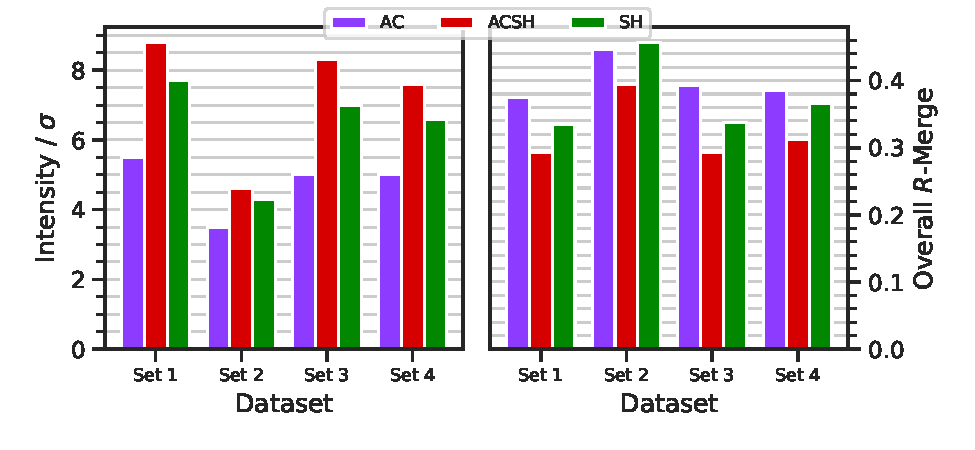
\includegraphics{plots/exp1/tlys_9_P6122/3p0_stats_grid.pdf}
    \caption{Merging statistics for Thermolysin 1 at 3.0 \unit{keV}.}
    \label{fig:tlys_9_3p0}
\end{figure}

\begin{figure}
    \centering
    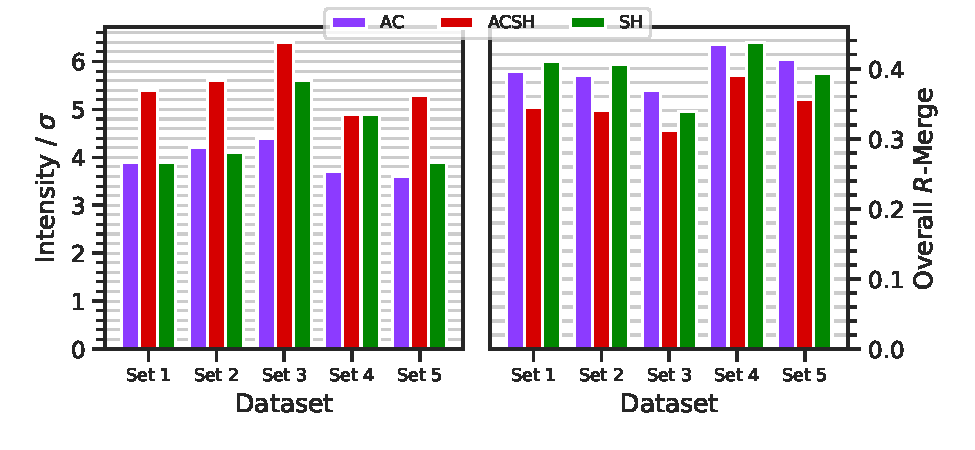
\includegraphics{plots/exp1/tlys_9_P6122/3p5_stats_grid.pdf}
    \caption{Merging statistics for Thermolysin 1 at 3.5 \unit{keV}.}
    \label{fig:tlys_9_3p5}
\end{figure}

\begin{figure}[h]
    \centering
    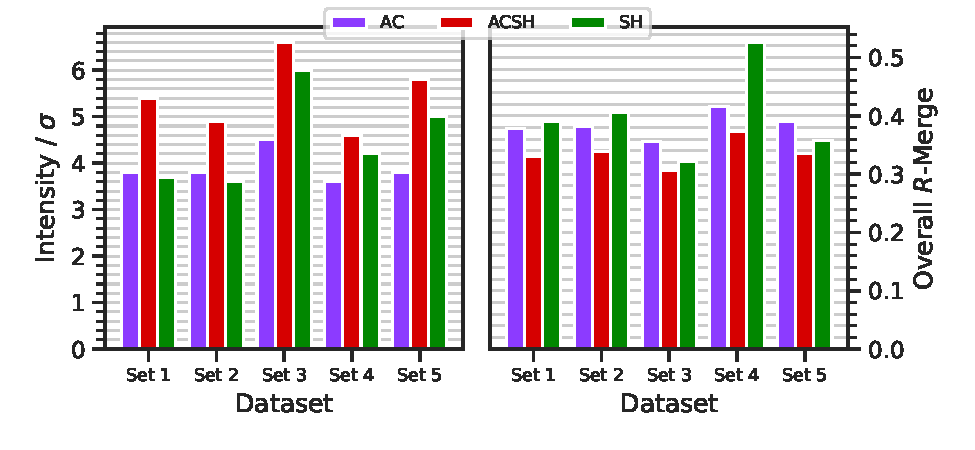
\includegraphics{plots/exp1/tlys_9_P6122/3p8_stats_grid.pdf}
    \caption{Merging statistics for Thermolysin 1 at 3.8 \unit{keV}.}
    \label{fig:tlys_9_3p8}
\end{figure}

Taking into account both the increase in $I/\sigma$ and decrease in $R_{merge}$, the merging statistics from Thermolysin 1 showed that \ac{acsh}, which combines tomography with spherical harmonics, was on average the best approach. While this was the case for every dataset of Thermolysin 1, some instances showed only a small improvement compared to \ac{sh}. Likewise, the standalone analytical approach was on average worse than \ac{sh} as well as \ac{acsh}.

Changes in energy are not expected to affect the reflection data; however, datasets that were collected subsequently on the crystal are more susceptible to radiation damage from longer exposure to the beam. If segmentation was then performed on a dataset collected early on in the tomography experiment, there can be discrepancies between the analytical model and a more-so radiation-damaged dataset.

%Following collection of reflection data, the AnACor results are used for structure refinement in Dimple, which generates anomalous density peaks for all the detected anomalous atoms and molecules based on the provided model. The results of Thermolysin 1

The merging statistics for individual datasets of Thermolysin 2 are shown in Appendix A3 in \cref{fig:tlys_2_3p0} and \cref{fig:tlys_2_3p5}. Since there were no clear outliers, all datasets with common energies were once again merged to produce the results shown in \cref{fig:tlys_2_stats}. Both parameters overwhelmingly show the same trend, with \ac{acsh} being the dominating correction method across all datasets and energies. This was corroborated with the $I/\sigma$ values and the R factors.
%that \ac{acsh} is once again the best correction method
%Results from Thermolysin 2 overwhelmingly show that \ac{acsh} is the dominating correction method, with $I/ \sigma$ highest and the R factors dipping across every dataset.

\begin{figure}
    \centering
    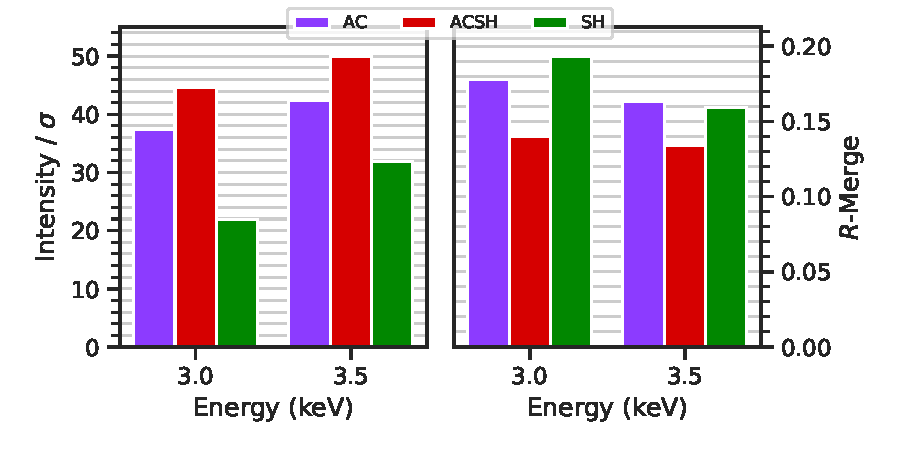
\includegraphics{plots/exp1/tlys_2_P6122/merged_stats.pdf}
    \caption{Merging statistics for Thermolysin 2 at 3.0 and 3.5 \unit{keV}.}
    \label{fig:tlys_2_stats}
\end{figure}

\begin{figure}
    \centering
    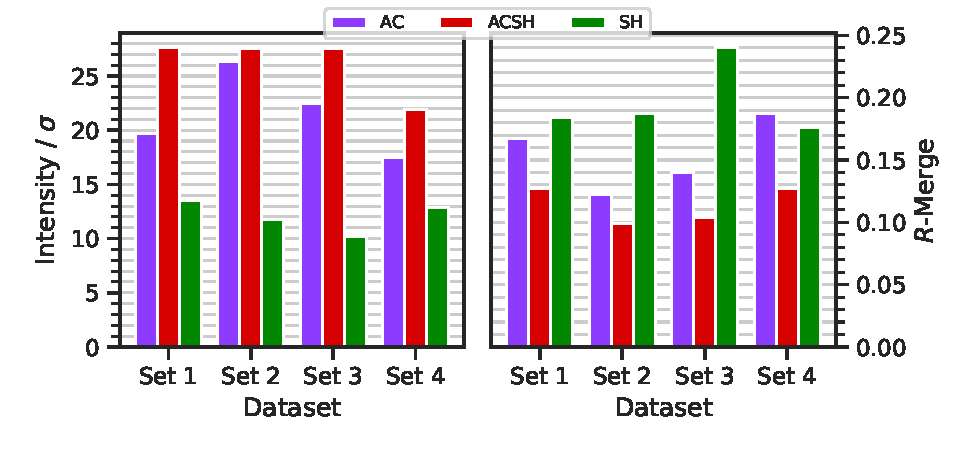
\includegraphics[width = 0.8\textwidth]{plots/exp1/tlys_2_P6122/3p0_stats_grid.pdf}
    \caption{Merging statistics for Thermolysin 2 at 3.0 \unit{keV}.}
    \label{fig:tlys_2_3p0}
\end{figure}

\begin{figure}
    \centering
    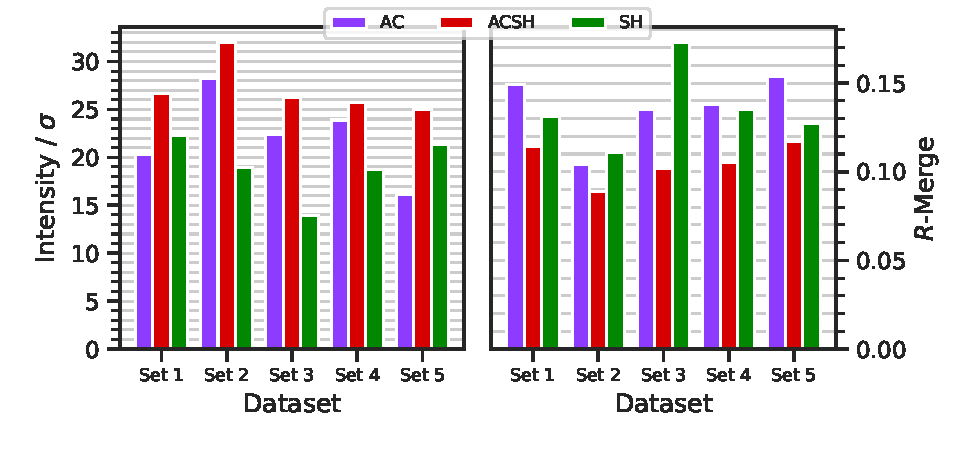
\includegraphics[width = 0.8\textwidth]{plots/exp1/tlys_2_P6122/3p5_stats_grid.pdf}
    \caption{Merging statistics for Thermolysin 2 at 3.5 \unit{keV}.}
    \label{fig:tlys_2_3p5}
\end{figure}

Following collection of reflection data, the AnACor results are used for structure refinement in Dimple to generate anomalous density peaks for all the detected anomalous atoms and molecules, based on the provided model. In thermolysin, the relevant anomalous groups are two methionine groups in positions 205 and 120 of the polypeptide chain of amino acid residuals \cite{CLAUDIO1984}, and a zinc atom. The results for individual datasets of Thermolysin 1 can be found in \cref{fig:tlys9_met_peaks_3p0,fig:tlys9_met_peaks_3p5,fig:tlys9_met_peaks_3p8,fig:tlys9_zn_peaks_3p0_3p5,fig:tlys9_zn_peaks_3p8}, and for Thermolysin 2 in \cref{fig:tlys2_met_peaks_3p0,fig:tlys2_met_peaks_3p5,fig:tlys2_zn_peaks} in Appendix A3.% and \cref{fig:tlys2_met_peaks_3p5}.

%While the heights of anomalous peaks are not a direct indicator of precision or quality, we can once again see that the coupled approach amplifies the detected anomalous signal from these groups.

Thermolysin crystallises in symmetry space group \textit{P}6\textsubscript{1}22. While processing in \textit{P}6\textsubscript{1}22 is therefore needed for obtaining reflection information, high symmetry crystals can still be processed in low symmetry groups, such as \textit{P}\textsubscript{1}, to observe the general merging statistics of the experiment, independent of reflections.
Datasets across the same energy processed in \textit{P}\textsubscript{1} were merged to increase the multiplicity of the low symmetry space group, and the results of processing Thermolysin 1 and Thermolysin 2 in \textit{P}\textsubscript{1} repeat the same trend seen for \textit{P}6\textsubscript{1}22.

\begin{figure}[h]
    \centering
    \begin{tabular}{cc}
    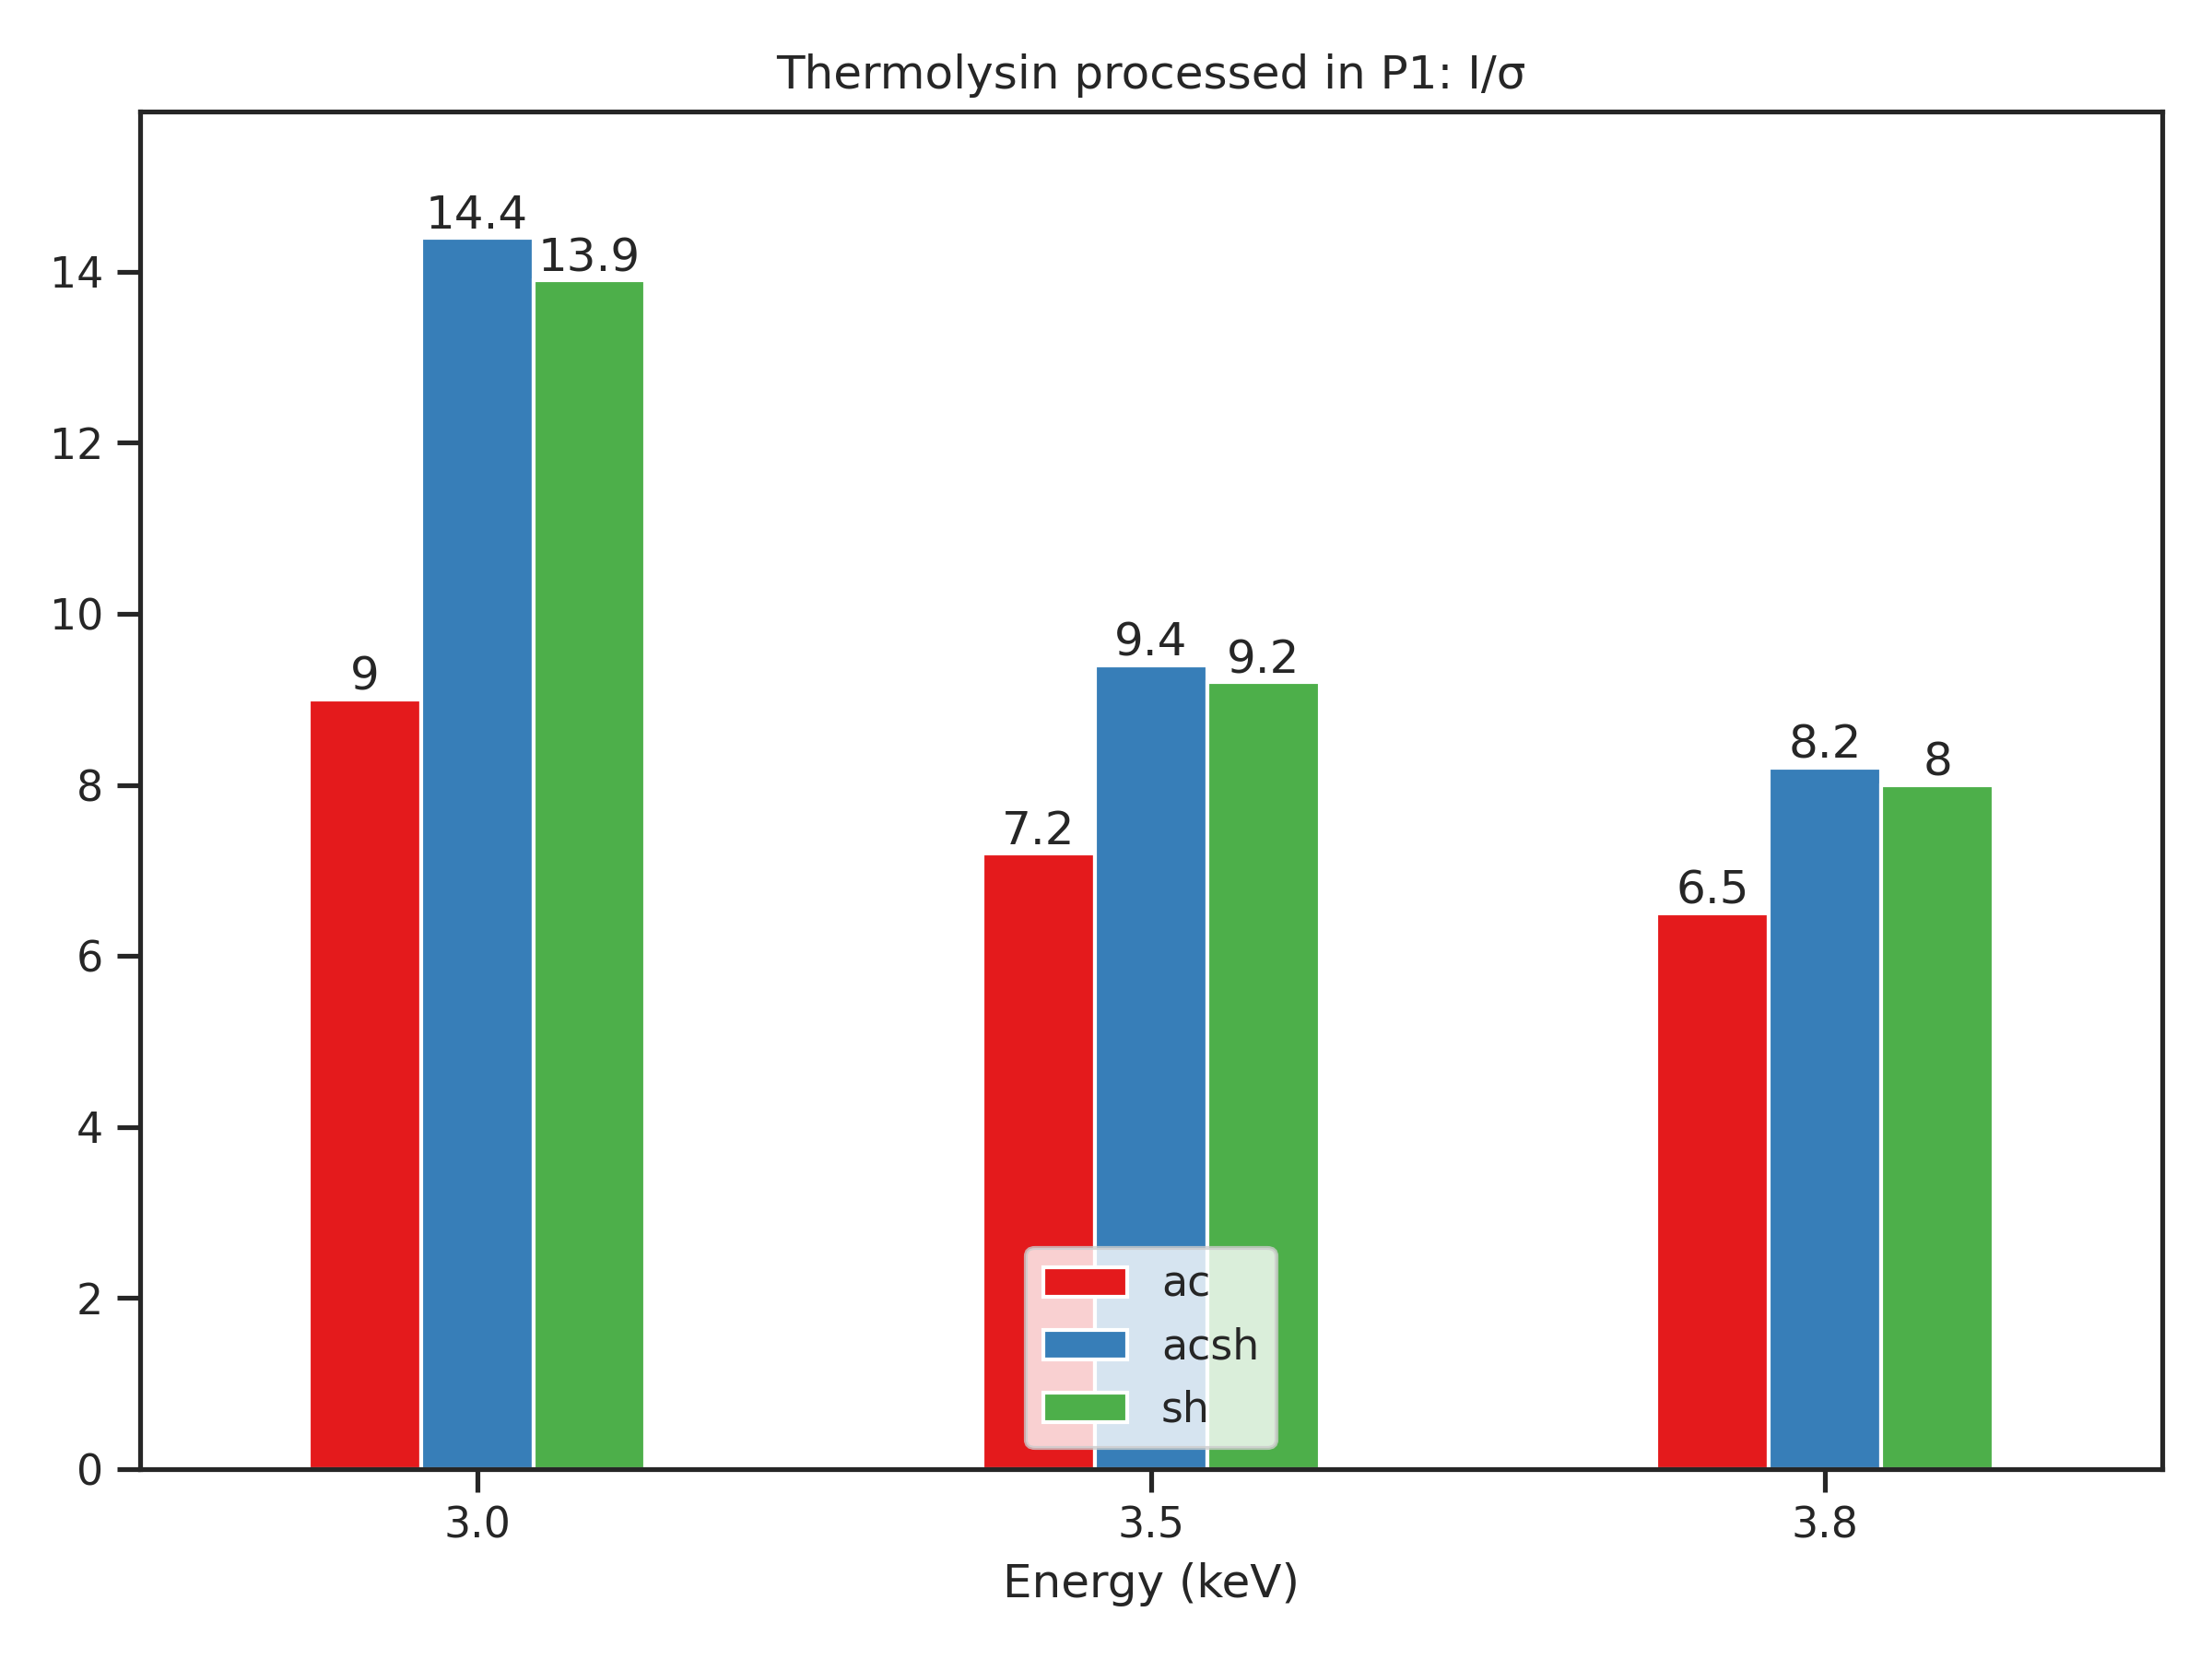
\includegraphics[width = 0.4\textwidth]{plots/exp1/tlys_9_P1/I_over_sigma.png} & 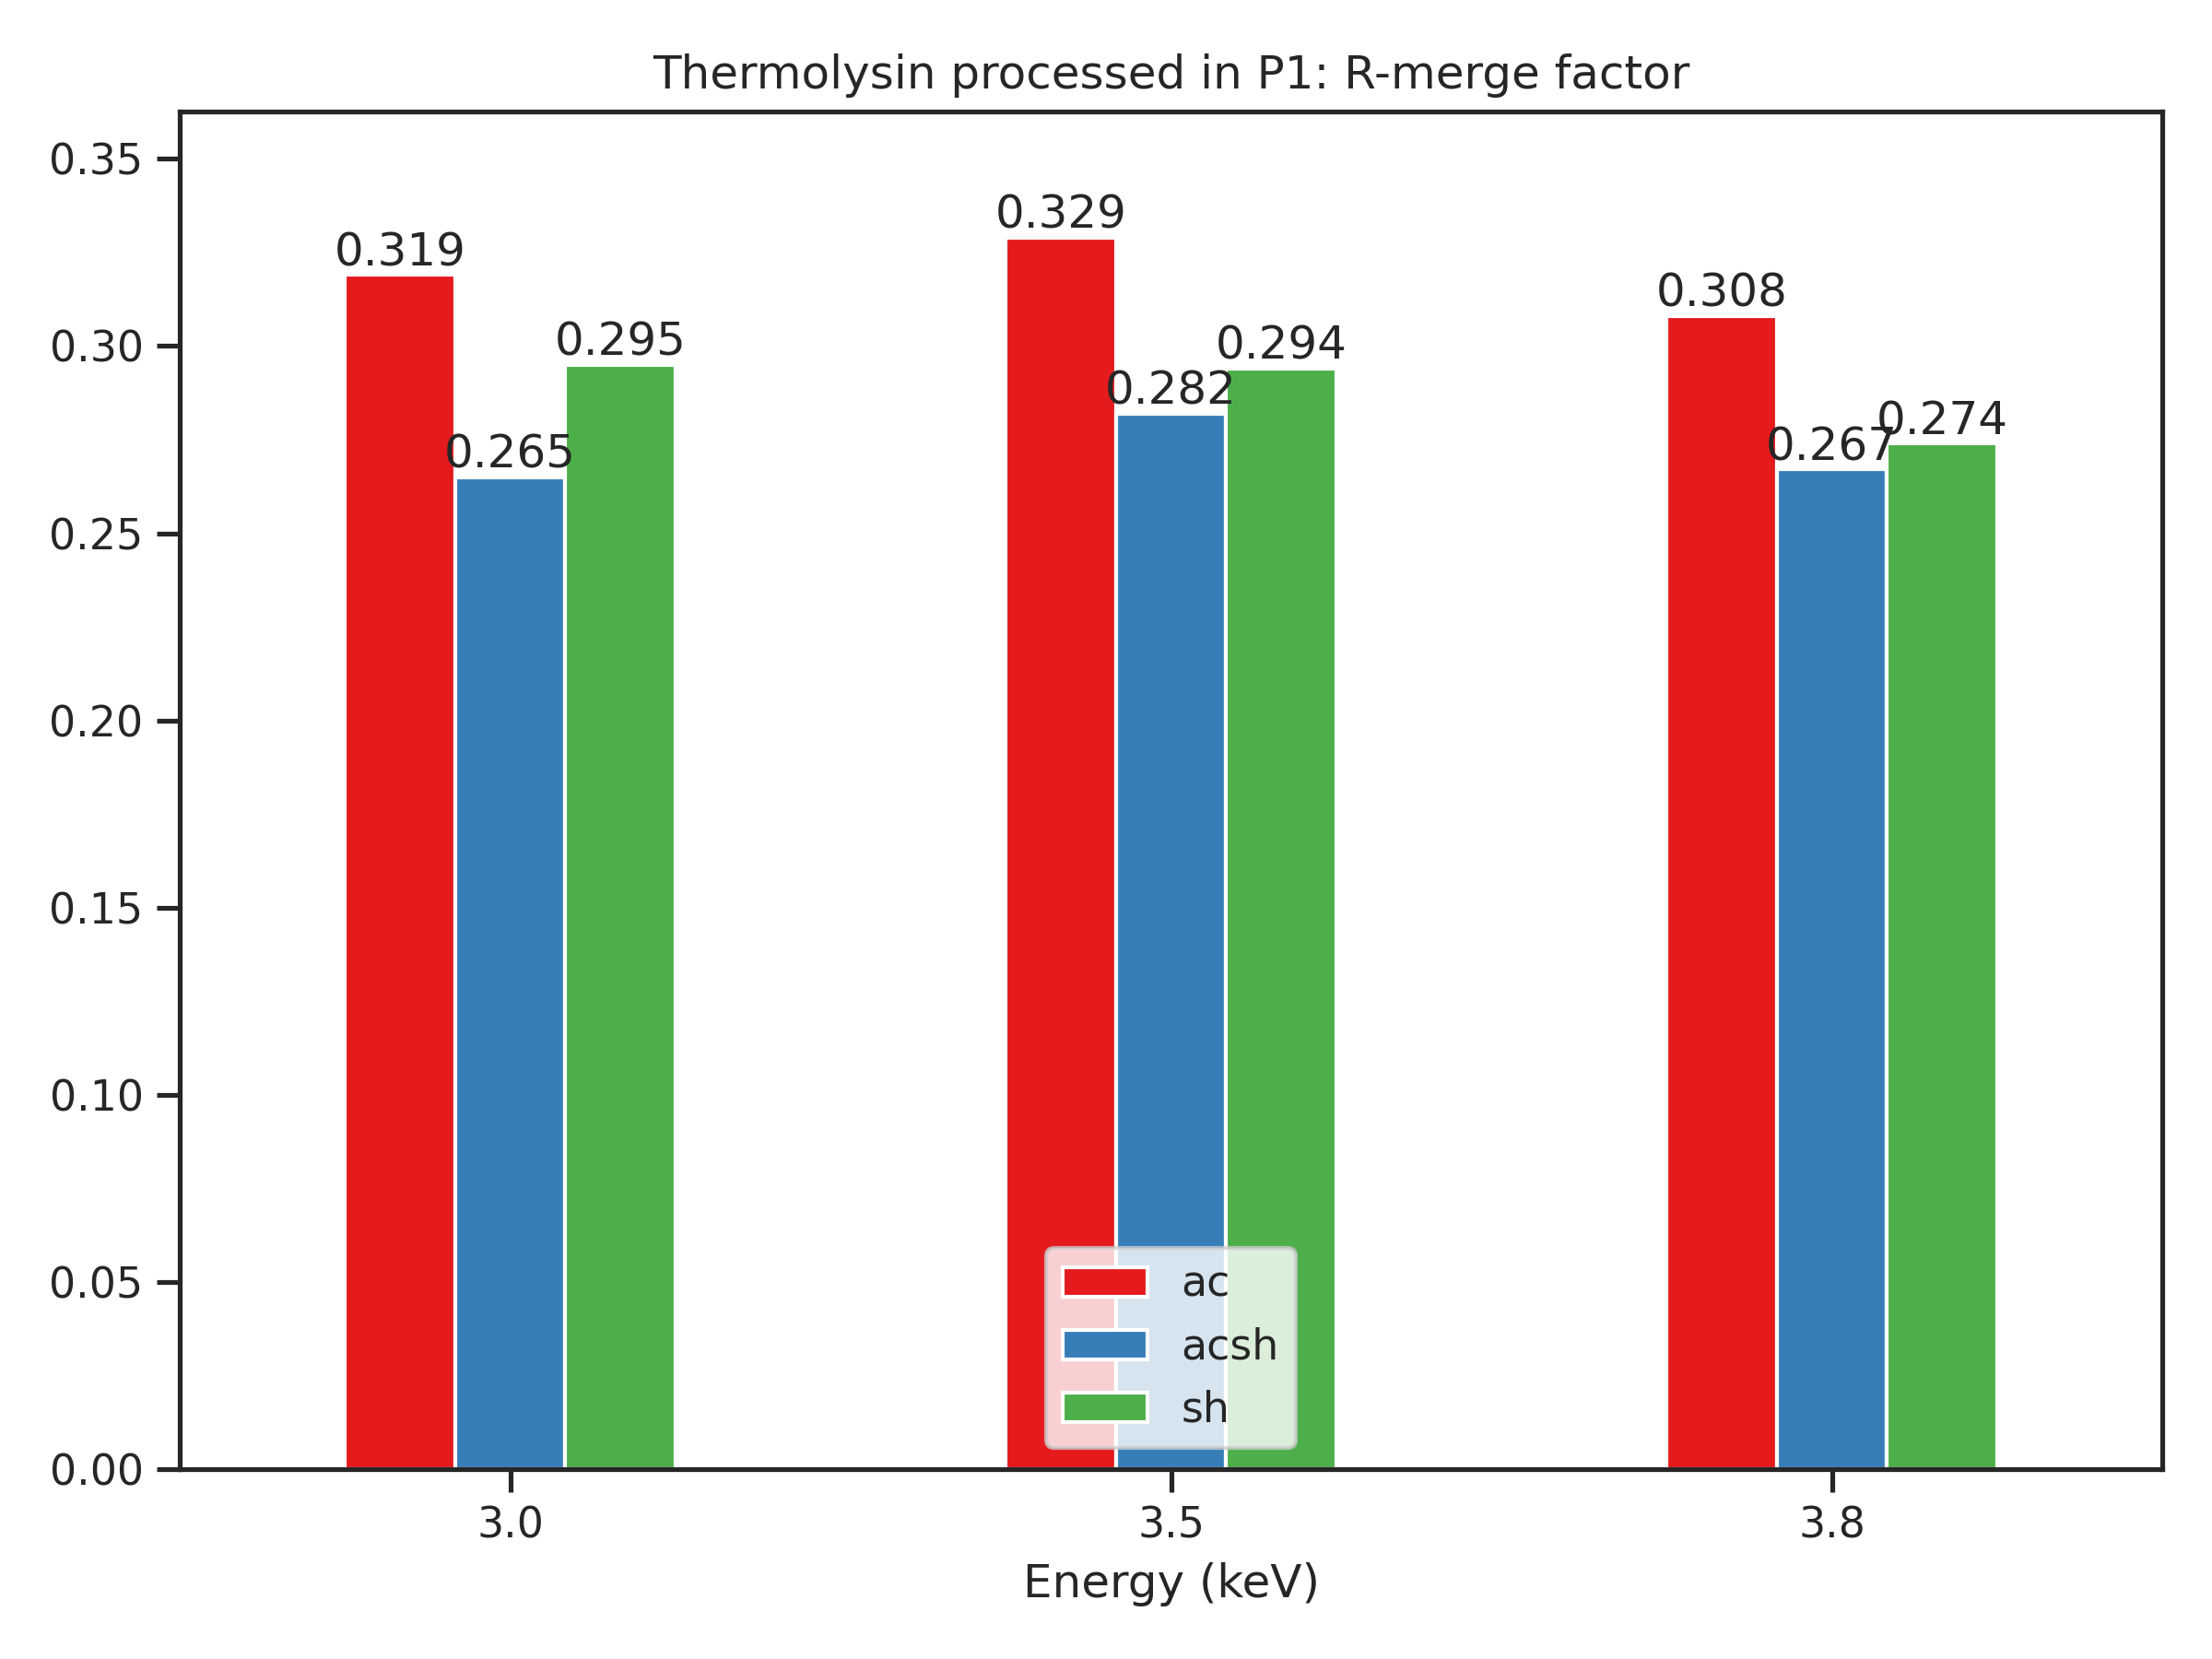
\includegraphics[width = 0.4\textwidth]{plots/exp1/tlys_9_P1/rmerges.png}
    \end{tabular}
    \caption{Merging statistics for Thermolysin 1 processed in $P_1$.}
    \label{fig:tlys_9_p1}
\end{figure}

\begin{figure}[H]
    \centering
    \begin{tabular}{cc}
    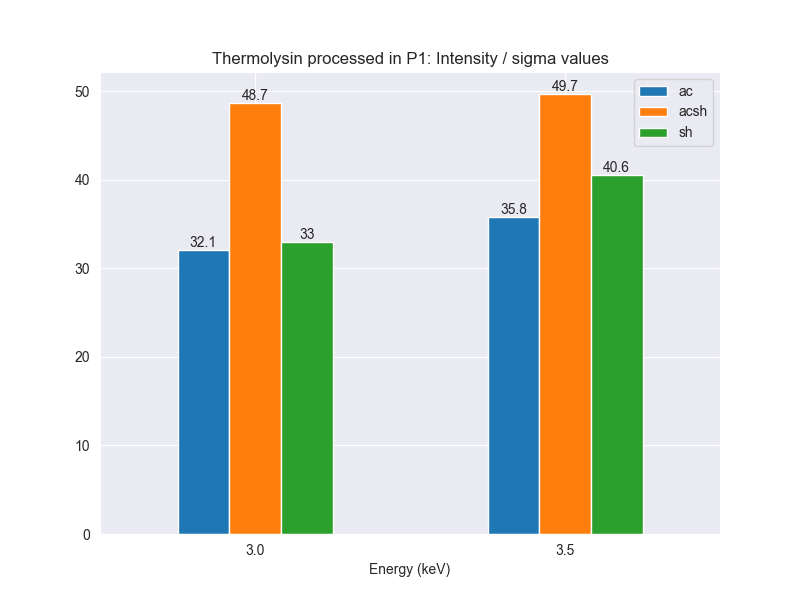
\includegraphics[width = 0.4\textwidth]{plots/exp1/tlys_2_P1/I_over_sigma.png} & 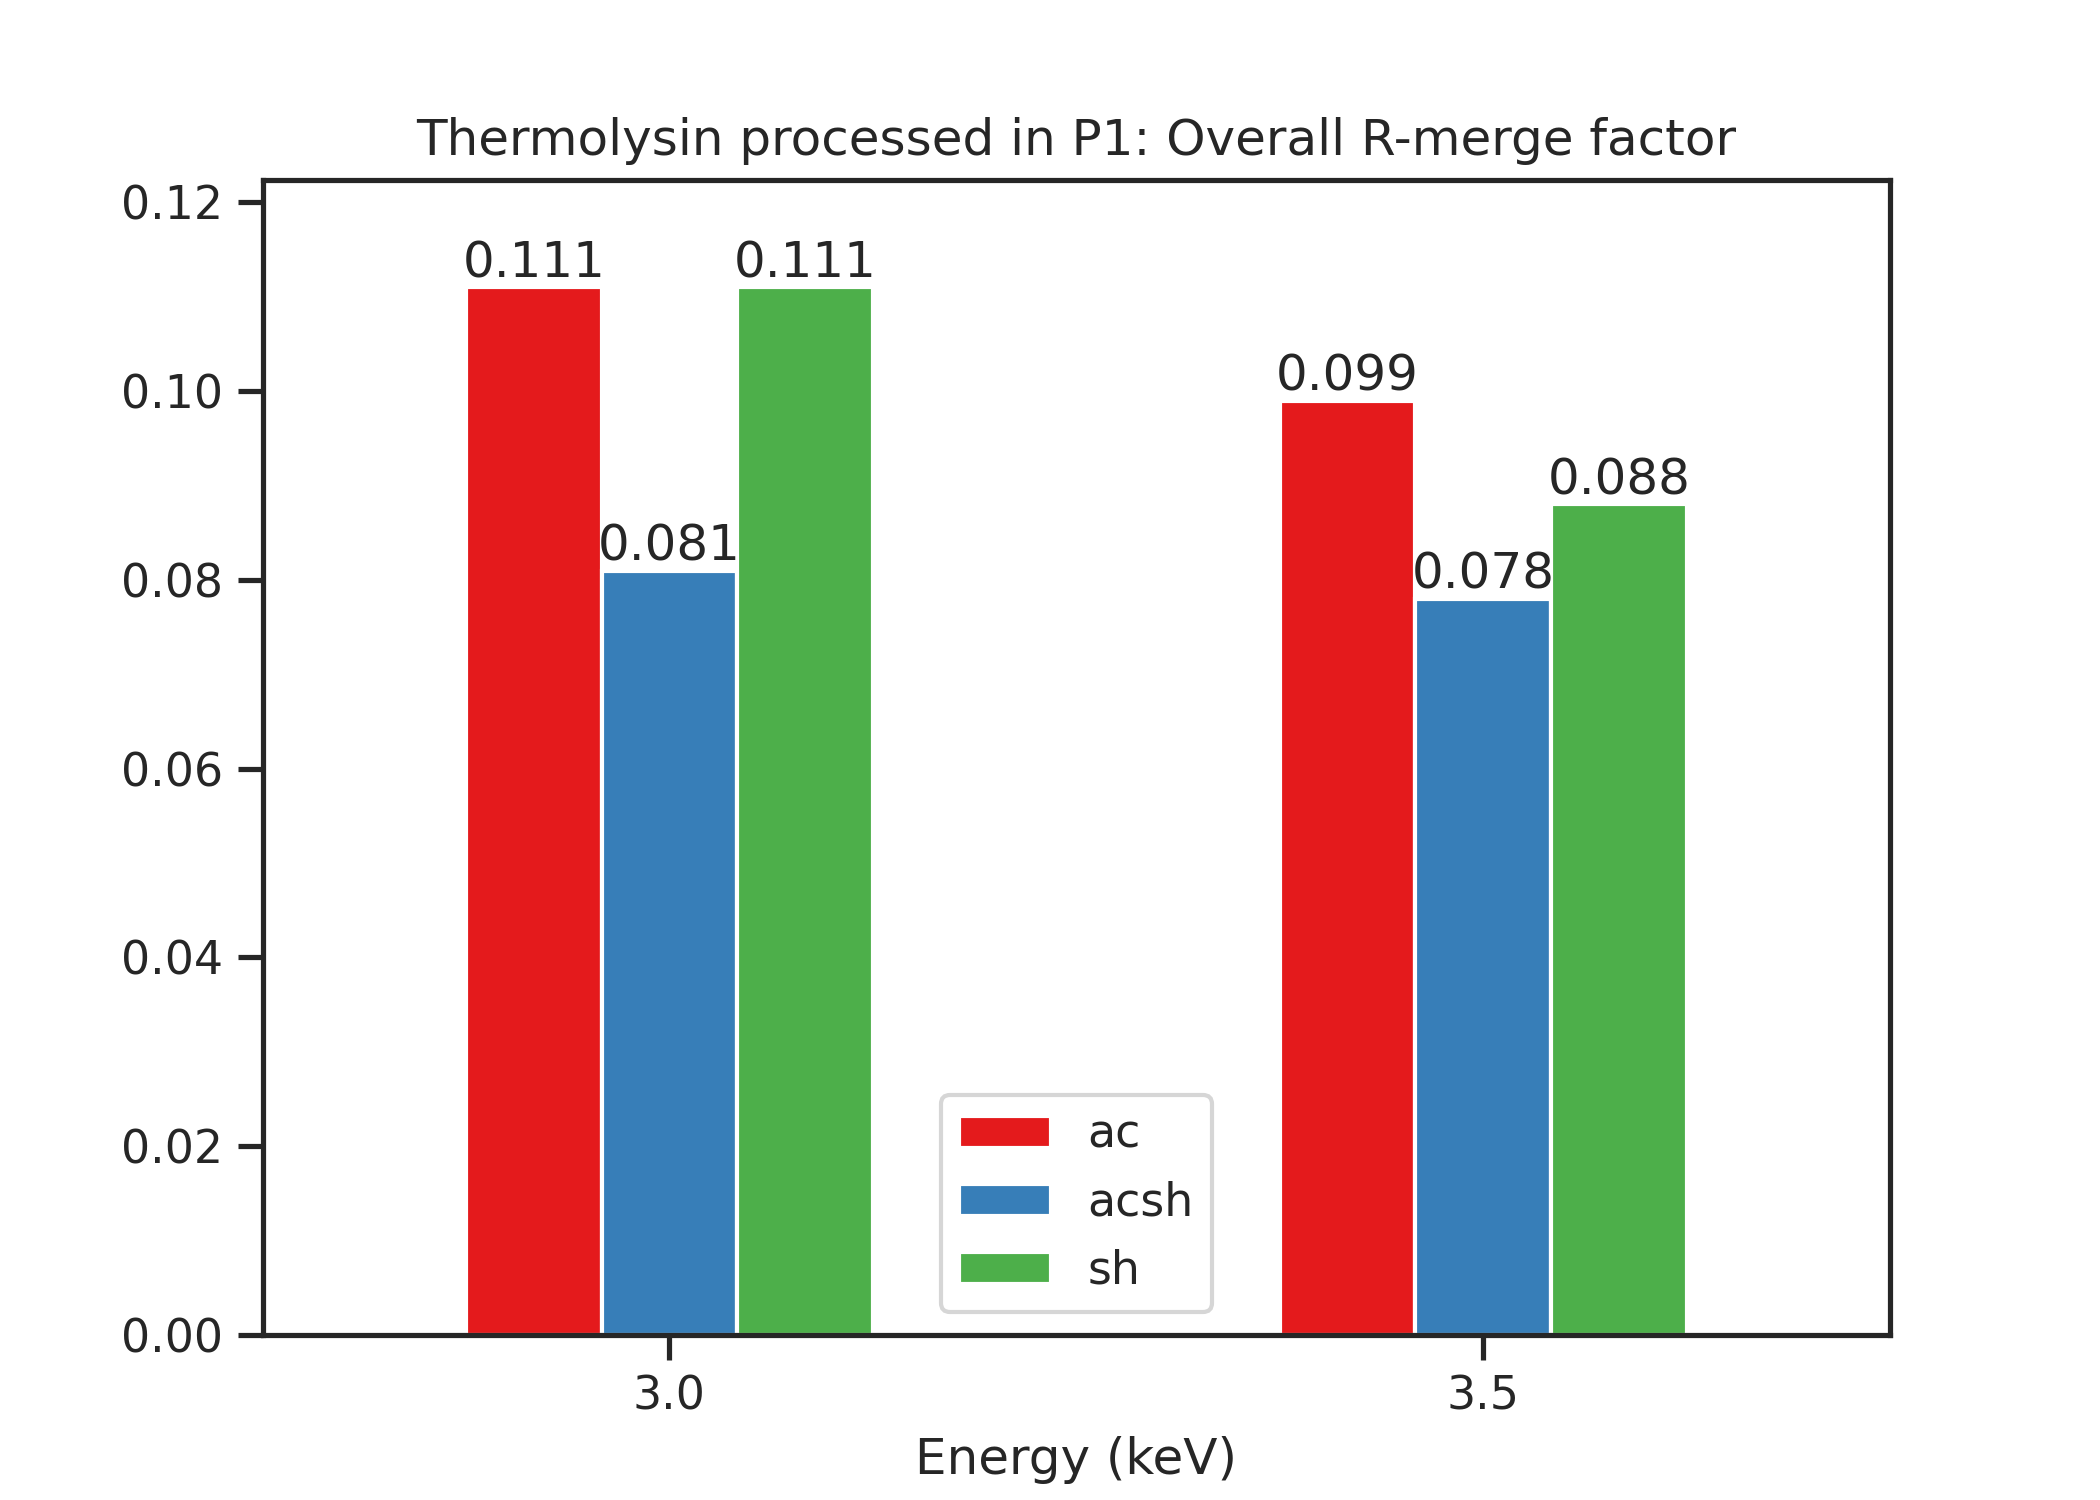
\includegraphics[width = 0.4\textwidth]{plots/exp1/tlys_2_P1/rmerges.png}
    \end{tabular}
    \caption{Merging statistics for Thermolysin 2 processed in $P_1$.}
    \label{fig:tlys_2_p1}
\end{figure}

\subsection{Analytically-corrected Tomography data in $f"$-refinement for ion identification}

%As of this year, I23 has established a new method of ion identification using anomalous scattering known as f" refinement. This protocol uses a programme known as Phenix which has a feature for estimating the f' and f" values of a given element based on the (mtz and pdb) of the collected crystal data. The f"-refinement is becoming a routinely-used feature of ion identification due to the long wavelength capabilities of the beamline. 

The reflection data from Thermolysin 2 that was produced across the three correction methods in the prior experiment were used in the platform known as \textit{phenix.refine} in Phenix. Phenix is a comprehensive software package for \ac{mx} structure determination; this particular platform allows for the refinement of absorption parameters $f'$ and $f"$ based on the reflection data and \ac{pdb} structure provided.

%As described in the methodology, t
The first stage of \textit{phenix.refine} uses the reflection data provided to produce a modified version of the molecular structure in \ac{pdb} format. This updated molecular structure is then used in the second stage with the same reflection data to estimate the theoretical $f'$ and $f"$ values of specified atoms that are believed to be in the structure. In the case of this experiment, $f'$ was fixed to its theoretical value for a given atom and energy, allowing for an experimental $f"$ to be refined. This value is then corroborated with the theoretical value to determine whether the atom type can be correctly identified.% test the ability of identifying atoms of sulphur and zinc in the crystal by determining their $f"$ peak.


\begin{figure}[h]
    \centering
    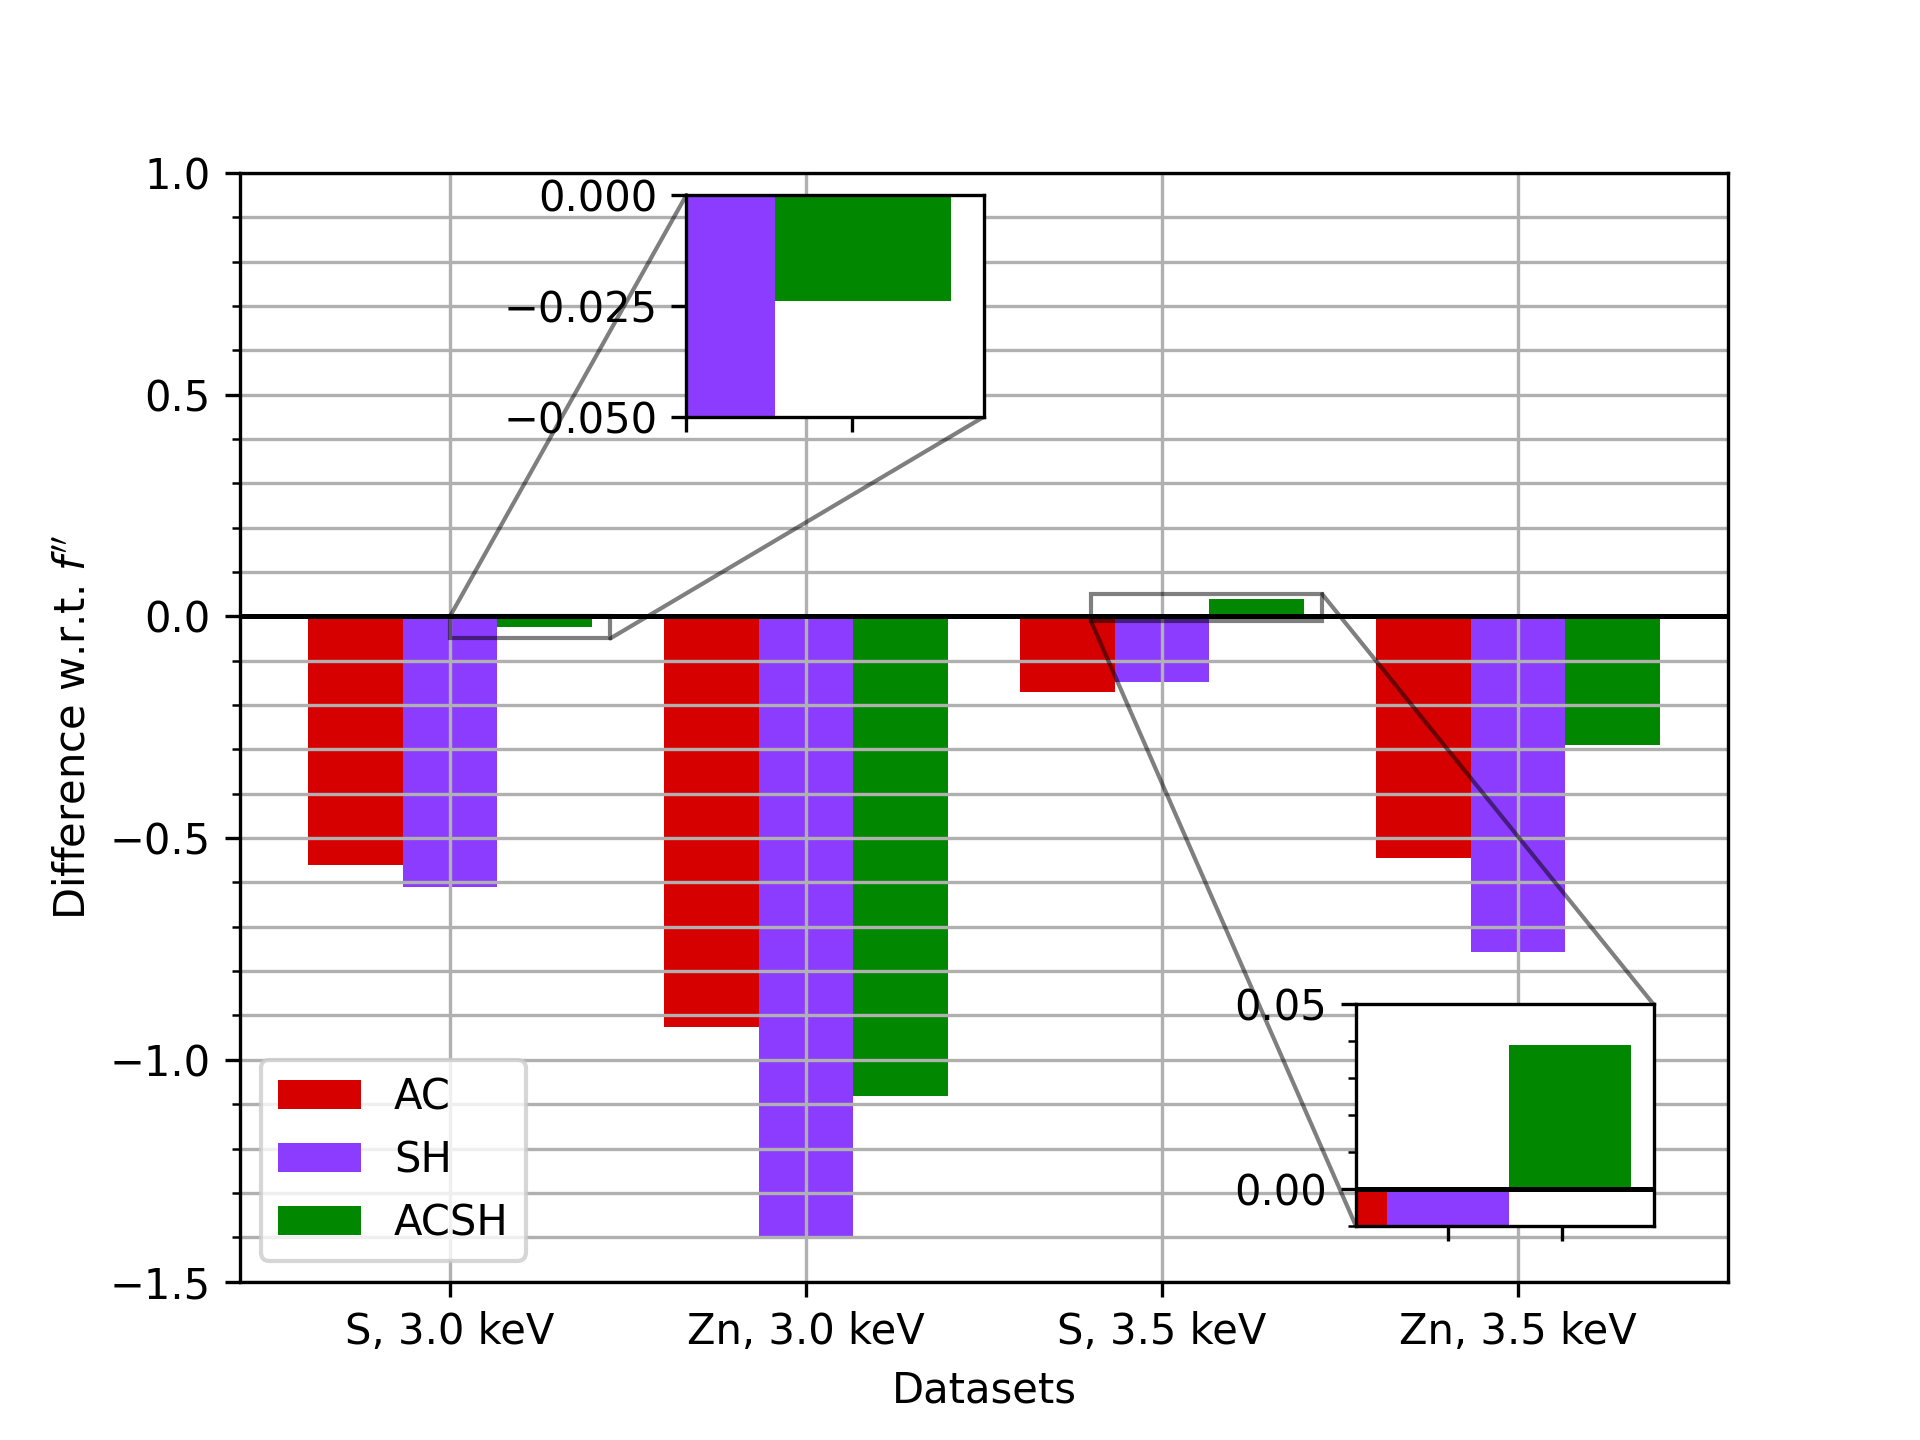
\includegraphics[width = 0.7\textwidth]{plots/phenix_plot_Pat.png}
    \caption{Difference with respect to theoretical $f"$ for atoms of sulphur and zinc in Thermolysin 2. Values obtained from \textit{Phenix.refine} in the Phenix software package for macromolecular structure determination.}
    \label{fig:phenix_plot}
\end{figure}

Results from Phenix refine for the six sets of reflection data of Thermolysin 2 (three methods across 3.0 and 3.5 \unit{keV}) are shown in \cref{phenix_table} and visualised in \cref{fig:phenix_plot}. The first most noticeable observation is that nearly every refinement underestimates the value of $f"$. It is also clear that refinement was generaly more precise at 3.5 \unit{keV} than at 3.0 \unit{keV}, and identification of the sulphur edge was more successful than that of zinc. Assuming the \ac{pdb} used correctly matched the residual atoms of thermolysin, this suggests that identification of zinc by the $f"$ refinement protocol cannot be achieved at such long wavelengths, and while it may improve data quality, the absorption corrections used here cannot sufficiently compensate for it. %could indicate that the zinc atom detected by Dimple is in fact not zinc, or

In the case of sulphur, it appears that this is no longer the case. While \ac{ac} fails to identify sulphur, comparison with \ac{sh} shows that \ac{acsh} brought the refined $f"$ value much closer to theoretical $f"$. At both energies, this approach successfully identifies the sulphur edge within 2 \% of the theoretical.%Another explanation, is the fact that the anomalous signal of sulphur is much stronger than that of zinc this reflection data was collected at 3.0 and 3.5 \unit{keV}, which are above the sulphur edge %which may indicate that the \ac{pdb} used did not sufficiently match the test crystals to correctly model the zinc atom.

Given that this experiment has only been performed on one crystal, it would be of interest to see whether this behaviour is seen again in $f"$-refinement at long wavelength with other crystals and atom types. %Another potential experiment would be to test if 

\subsection{Analytical tomography corrections with laser-shaped samples}

Following the experiments that showed the successes of tomographic reconstruction and segmentation corrections, the next question to investigate was about its compatibility with another form of absorption correction. Laser-shaping has previously been used in cryogenic \ac{mx} to remove the non-diffracting material contributing to background noise, thus improving the diffraction quality and likewise the standard \ac{sh} absorption corrections that only assume for the diffracting material in a sample.

Both X-ray tomography and laser-shaping have therefore proven to improve the quality of low-energy diffraction, but their combined effects had not yet been explored. In the following experiment, two crystals of insulin and two of proteinase K were used for a preliminary test of what this combined effect would look like. Each protein experiment had one control crystal and one that was laser-shaped to remove a majority of the loop and solvent. These samples were then segmented to produce the models shown in \cref{avizo_insulin} and \cref{avizo_proteinasek}.

The laser-shaped samples were ablated with the intention to make a spherically shaped crystal that was, ideally, the only material entity. While the crystals were spherical in shape, the size of the crystals used limited the samples to still containing some mother liquor. The laser-shaped samples were therefore not \textit{perfect} crystal spheres, but were nonetheless entirely void of loop material.

The merging statistics obtained from this experiment tell somewhat different stories, depending on the protein. 

\begin{figure}[h]
    \centering
    \begin{tabular}{cc}
    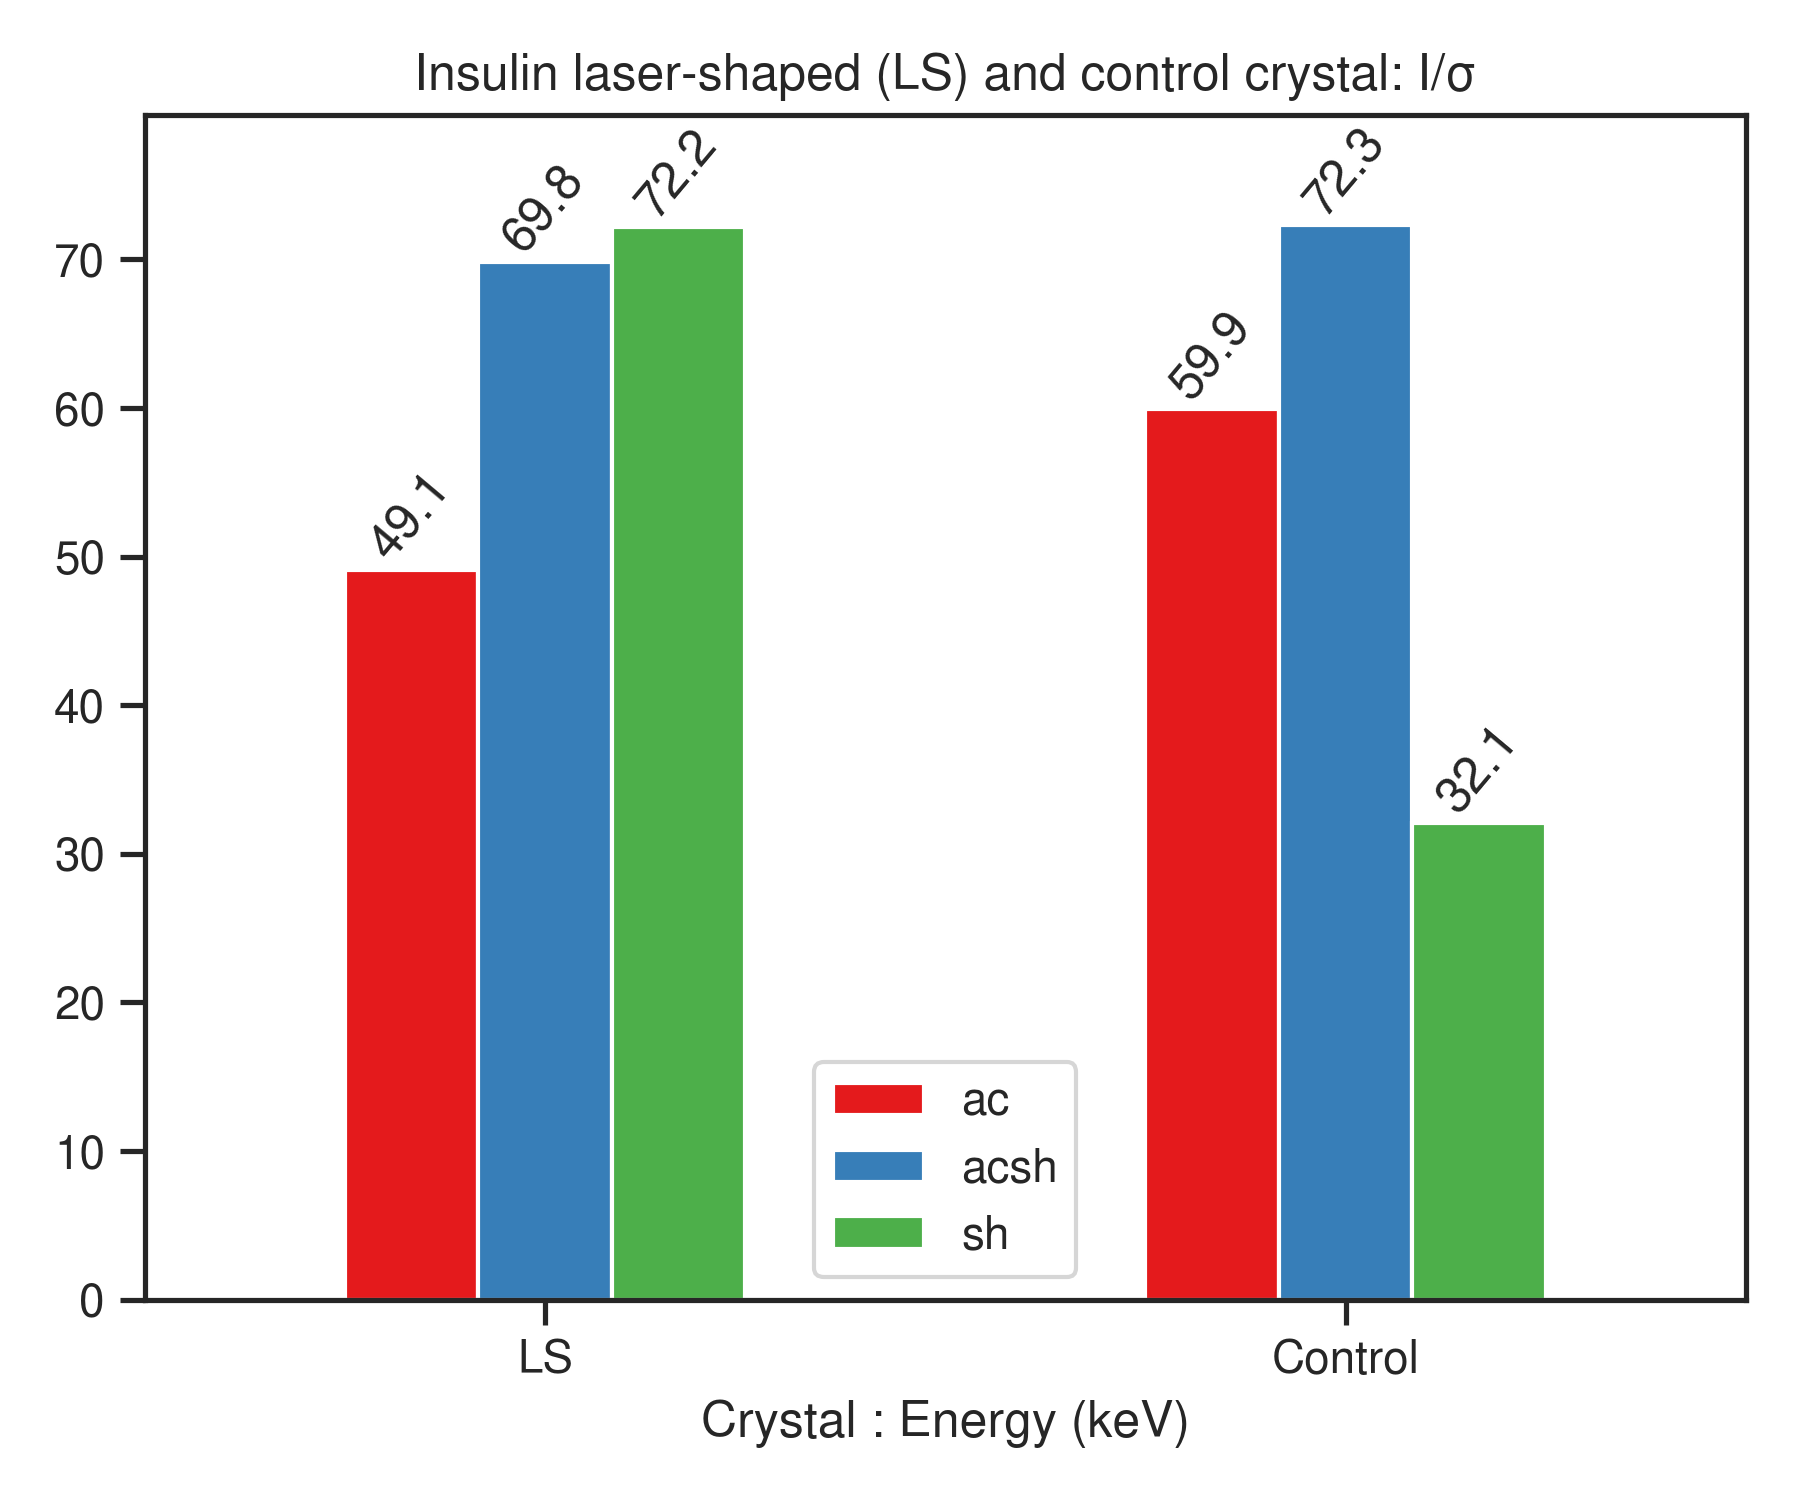
\includegraphics[width = 0.5\textwidth]{plots/exp2/ins_I_over_sigma.png} & 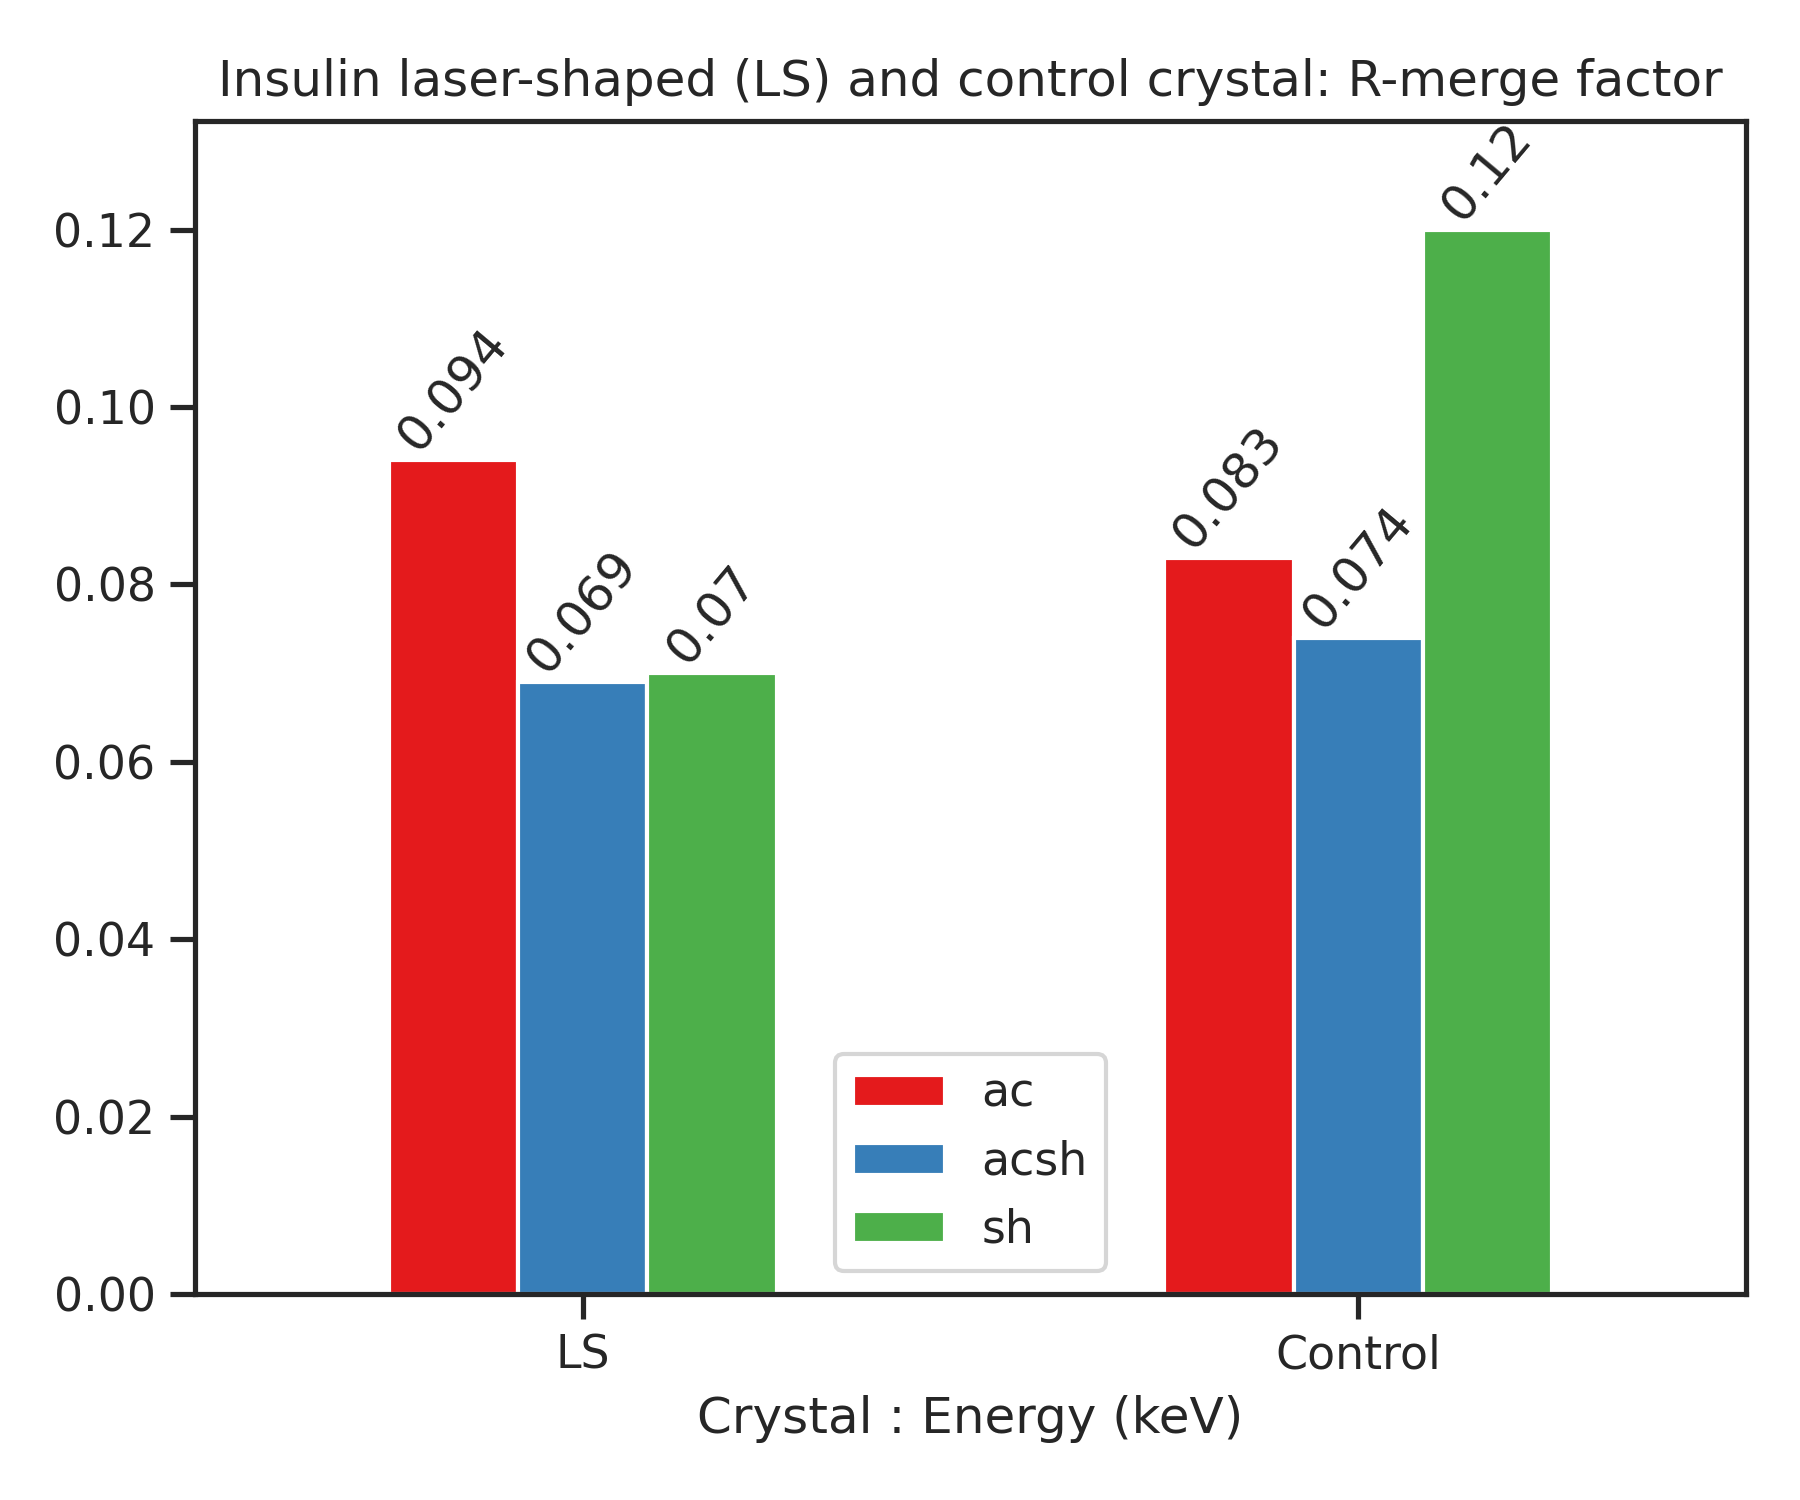
\includegraphics[width = 0.5\textwidth]{plots/exp2/ins_rmerges.png}
    \end{tabular}
    \caption{Merging statistics for the laser-shaped and control crystals of insulin at 3.0 \unit{keV}.}
    \label{fig:insulin}
\end{figure}

\begin{figure}[h]
    \centering
    \begin{tabular}{cc}
    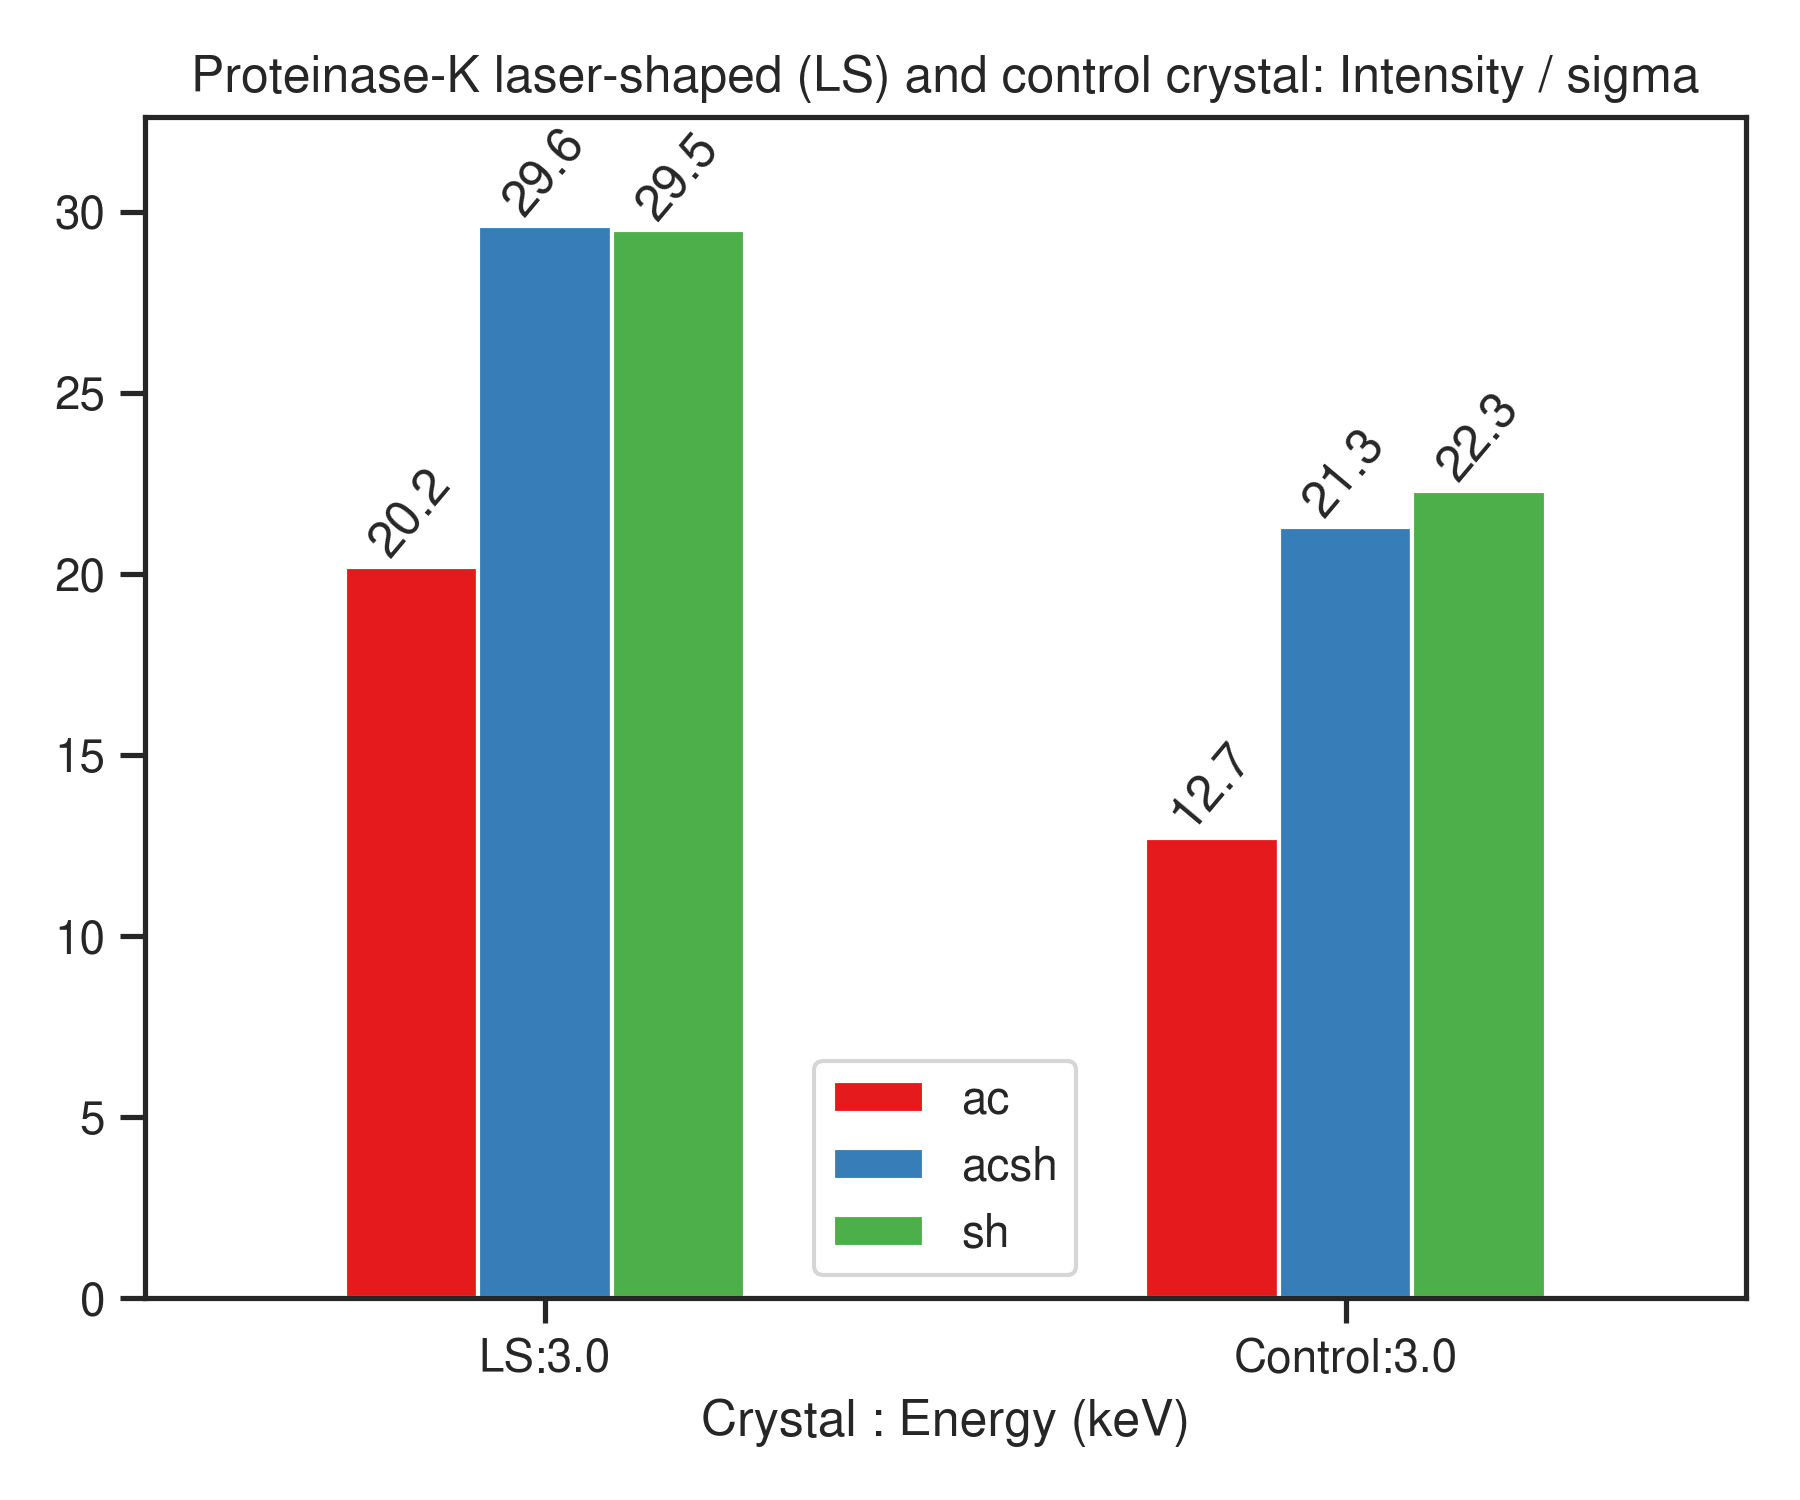
\includegraphics[width = 0.5\textwidth]{plots/exp2/prot_I_over_sigma.png} & 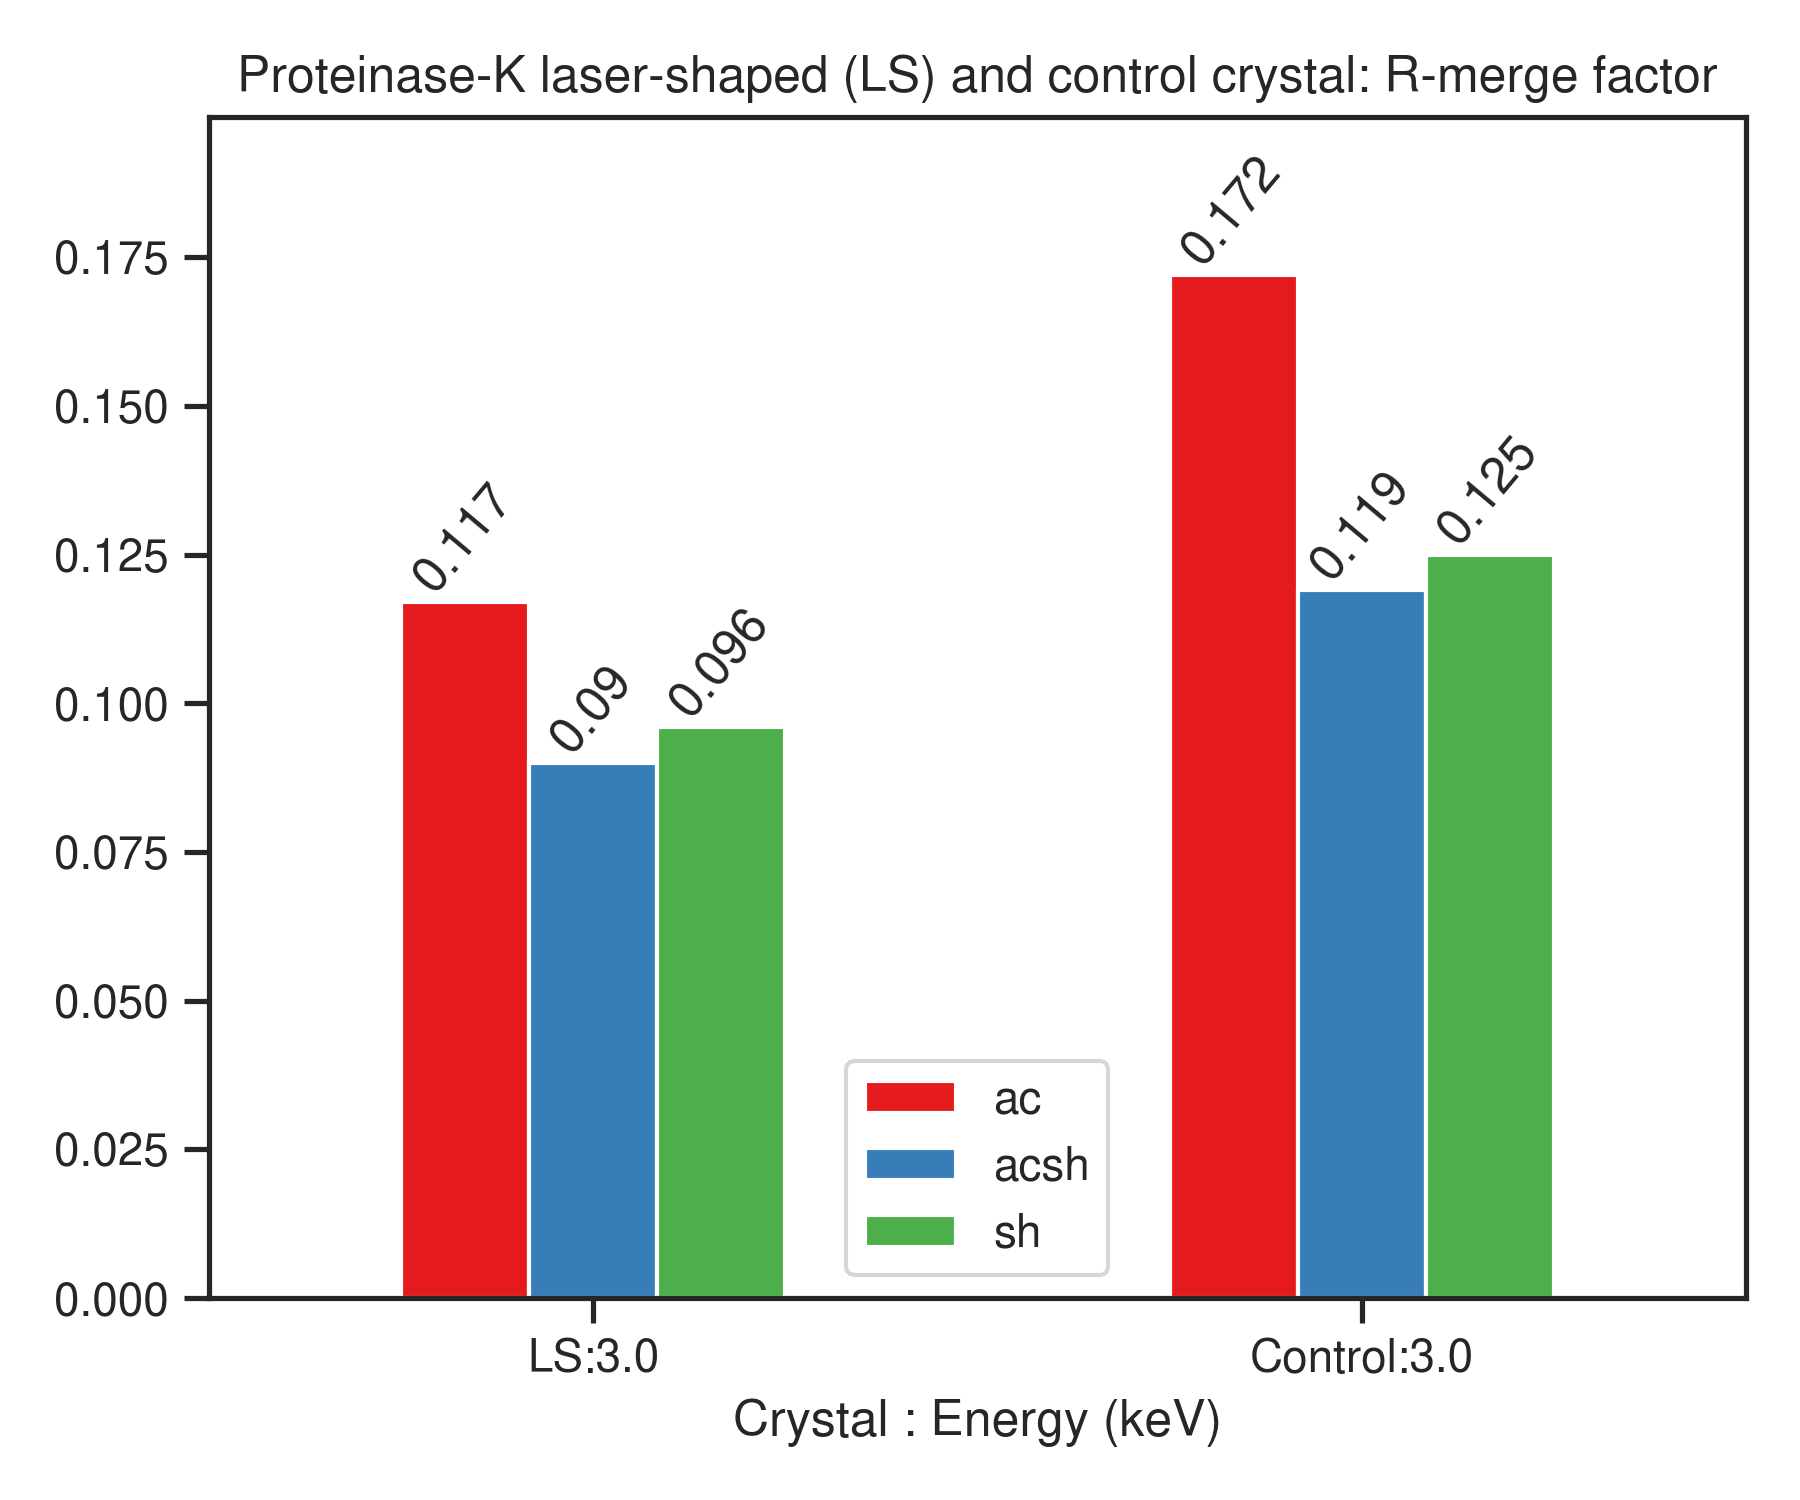
\includegraphics[width = 0.5\textwidth]{plots/exp2/prot_rmerges.png}
    \end{tabular}
    \caption{Merging statistics for the laser-shaped and control crystals of Proteinase K at 3.0 \unit{keV}.}
    \label{fig:proteinasek}
\end{figure}

The insulin crystals, shown in \cref{fig:insulin}, suggest there is little to no change in the \ac{acsh} approach between the laser-shaped and control. \Ac{sh}, on the other hand, experiences a huge boost from laser-shaping. This is to be expected for more than one reason; spherical harmonics assume a spherical shape of the crystal, and therefore model the effects of absorption more reliably with the laser-shaped sample; likewise, with \ac{sh} unable to account for non-diffracting material in the sample, the removal of most thereby leads to better diffraction and better empirical models.

A surprising feature of the insulin results is the fall in \ac{ac} from control to laser-shaped. While there is no reason for \ac{ac} to be improved from laser-shaping as the physical is anyway accounted for in detail, it is unusual for analytical calculations to worsen. It is believed that this discrepancy can be attributed to the surface of laser-shaped insulin, seen in \cref{avizo_insulin}, which was covered by bubbles of what was presumed to be liquor. Aside from the fact that these bubbles contribute to background noise while not contributing to diffraction, the high contrast of this surface made detailed segmentation especially challenging. The limitations on the analytical model could therefore be the cause. % of this

Results from proteinase K, shown in \cref{fig:proteinasek}, suggest there is a noticeable improvement in laser-shaping compared to standalone tomography. This is unexpected when compared to the trend seen with insulin. The control, however, does not follow the expected behaviour either; with \ac{sh} and \ac{acsh} being nearly identical among both parameters. This could be attributed simply to poor diffraction; however, more data must be analysed to reach a conclusive picture of what is happening.

A common feature to both proteins is that in the case of the laser-shaped sample, \ac{acsh} and \ac{sh} remain nearly identical across both parameters.
This suggests that, while tomography-based reconstruction and laser-shaping are both successful absorption corrections in their own right, the effects of combining these at long wavelengths remain unchanged.

Previous studies done on tomography-based analytical corrections have focused on low-symmetry space groups, such as $P_1$, $P_2$, and $C_2$; as it was believed that high symmetry crystals with a naturally high multiplicity would not benefit from geometry-dependent analytical approaches. Given that thermolysin, and insulin in particular, are both high-symmetry, the preliminary results from these crystals would suggest that the benefits of analytical corrections are not limited to only low-symmetry space groups. This is particularly relevant for future applications of this technique in soft-X-ray experiments.

%Testing tomo on lysosyme to try to detect sodium anomalous signal

%Mention LASER-shaping already worked on identifying magnesium in topoisomerase crystals. Hypothesis: tomography can do the same

\subsection{Detecting sodium in lysozyme with analytical tomography corrections}


\subsection{Errors and Improvement}

Faults in the absorption coefficients are particularly sensitive to the thresholding in AnACor that predicts the location of a material. While the alignment of the threshold tends not to be a problem for segmented datasets, datasets with different flat fields that reuse the same segmentation model have recently been having minor displacement problems in the newest version of AnACor. Indications of coefficients being overestimated or underestimated, such as with Cld and Ompk, can be attributed to these problems.  

While it is unclear whether this affects the quality of results in this project, further steps must be taken to resolve the material selection and ensure analytical pathways are computed precisely.

Current efforts are being put forward to developing an automatic segmentation procedure at I23. This would significantly boost the speed of data processing jobs in tomography, as segmentation is the most meticulous aspect of the routine.

%Faults in anacor thresholding, particularly at processing datasets collected at multiple energies

%segmentation at high contrast

%There are several challenges associated with the segmentation of X-ray data of protein crystals.